\section{Same Flavor final state}\label{sec:SF}
The analysis if the same-flavour final state $\mathrm{W^+W^-}\to \mu^{\pm}
\mu^{\mp}  2\nu$ and  $\mathrm{W^+W^-}\to e^{\pm} e^{\mp}  2\nu$ is described
in this section. \\

\subsection{Signal region}
Events are requested to pass single or double lepton triggers and all the
physics objects definitions are the same as in the OF analysis.
The final state consists of two well identified electrons or two muons with
$p_T >$ 20 GeV, opposite charge, and large missing transverse energy from the undetected neutrinos.\\
In addition to the backgrounds described for the OF final state, the
background from $\mathrm{DY}\to \mu^{+} \mu^{-}$ and
$\mathrm{DY}\to e^{+} e^{-}$ is very large in this final state.
Indeed, due to this very large background, the SF analysis only targets the
VBF topology, where the DY background is suppressed by the tight 
jet requirements. In addition, an invariant mass of the two leptons larger
than 120~\GeV is requested.
The full selection, defined as the ''WW SF selection'', is :

\begin{itemize}
\item Two isolated leptons with same flavor and opposite charge ($\mu ^{\pm} \mu^{\mp}$ and $e^{\pm} e^{\mp}$);
\item $p_T$ of the leading and trailing lepton $>$ 20 GeV;
\item Third lepton veto: veto events if a third lepton with $p_T  >$ 10 GeV;
\item  $m_{\ell \ell} >$ 120 GeV 
\item $p_T^{\ell \ell} >$30 GeV;
\item MET $>$ 50 GeV;
\item $m_T^I >$ 100 GeV;
\item At lest 2 jets non b-tagged (according to cMVAv2 loose WP) with $p_T >$ 30 GeV.
\item $\Delta \eta_{jj} > 3.5$;
\item $m_{jj} >$ 500 GeV;;
\end{itemize}


Similarly to the OF analysis, the signal is extracted from a template fit of
the $m_T^I$ distribution.
The $m_T^I$ distributions has the following binning:

\begin{itemize}
\item {\bf VBF}, [100,150,200,250,300,350,400,450,500,600,700,1000];
\end{itemize}
where the first number represents the lower edge of the first bin while the other numbers represent the upper edges. The last bin is an overflow bin. 
The binning has been chosen in order to have at least 10 expected Top-backgrounds event and at least 10  expected  Drell-Yan events in each bin of the template.\\
The distributions for the signal region, still blinded, of $m_T^I$,  $m_T^H$,
$m_{\ell \ell}$ and $m_{jj}$ are presented for the $\mu ^{\pm} \mu^{\mp}$ and $e^{\pm} e^{\mp}$ 
case in Figs.~\ref{fig:mti_sigSFee} and \ref{fig:mti_sigSFmm}.




\begin{figure}[htbp]
\centering
\subfigure[$m_T^I$]{
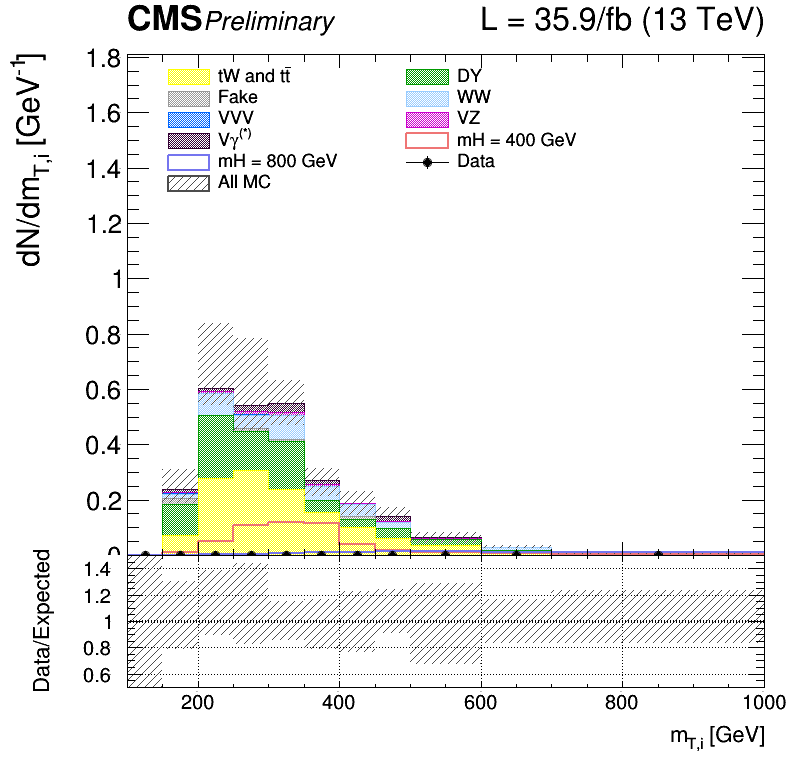
\includegraphics[width=0.45\textwidth]{Figs/SF_SR_Blind/cratio_hwwhm_13TeV_e_e_2j_VBF_mTi.png}
}
\subfigure[$m_T^H$]{
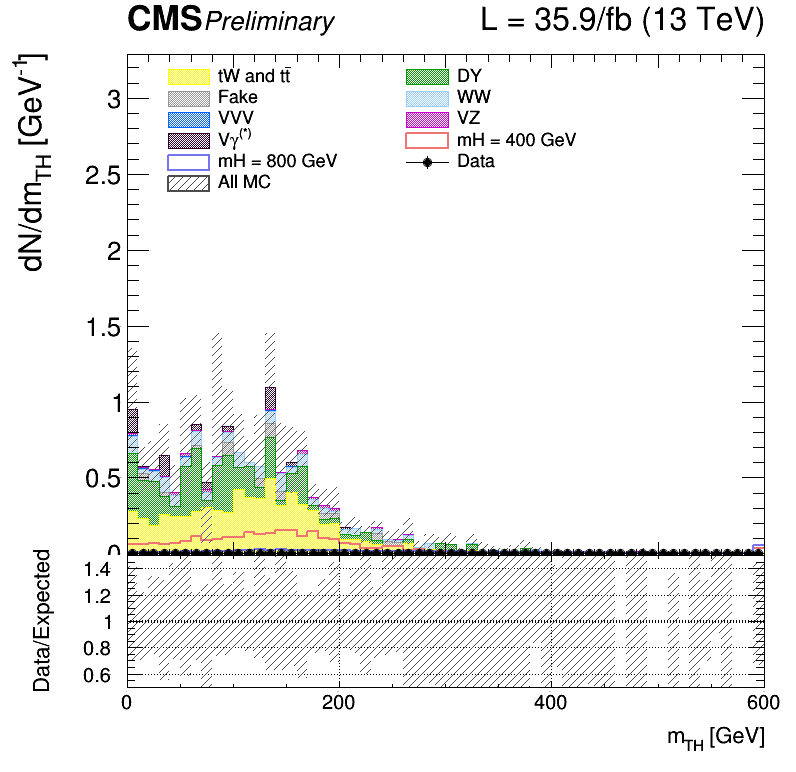
\includegraphics[width=0.45\textwidth]{Figs/SF_SR_Blind/cratio_hwwhm_13TeV_e_e_2j_VBF_mth.png}
}
\\
\subfigure[$m_{\ell \ell}$]{
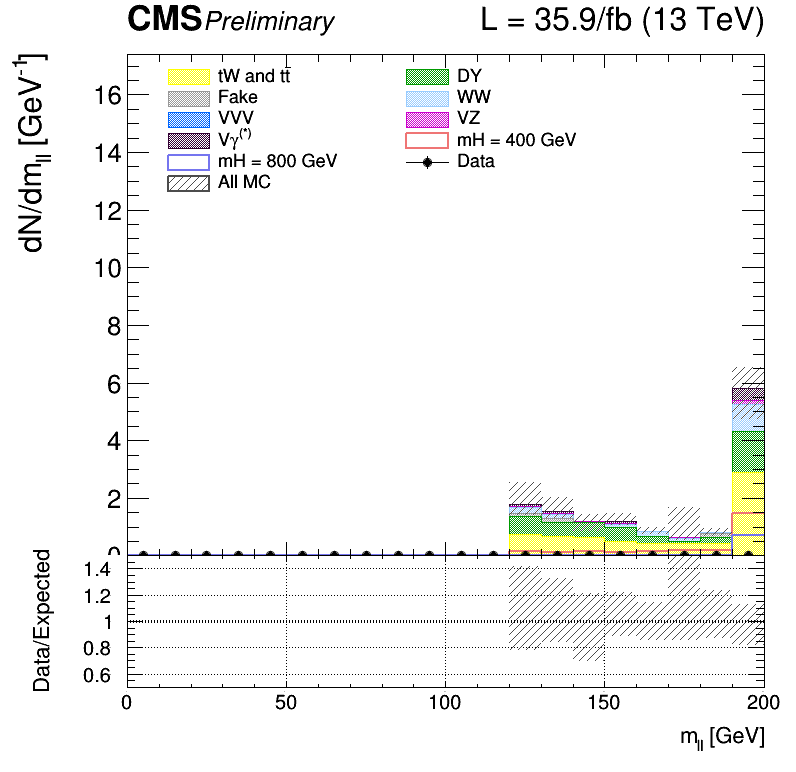
\includegraphics[width=0.45\textwidth]{Figs/SF_SR_Blind/cratio_hwwhm_13TeV_e_e_2j_VBF_mll_DY.png}
}
\subfigure[$m_{jj}$]{
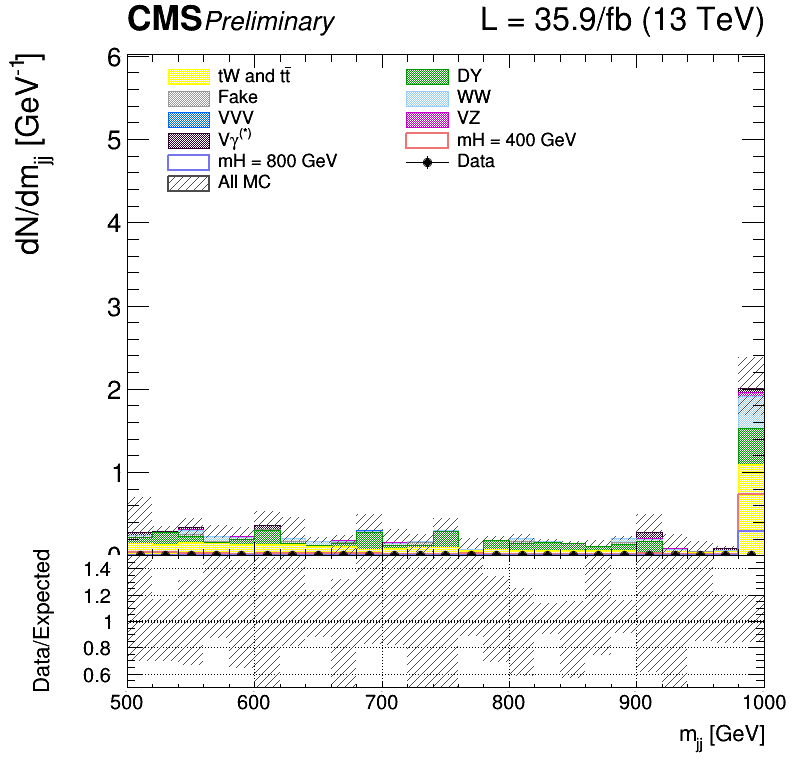
\includegraphics[width=0.45\textwidth]{Figs/SF_SR_Blind/cratio_hwwhm_13TeV_e_e_2j_VBF_mjj_DY.png}
}
\caption{Distributions  $m_T^I$, $m_T^I$, $m_T^H$, $m_{\ell \ell}$ and $m_{jj}$ in the signal region $e^{\pm} e^{\mp}$ case. Two different signal hypothesis corresponding to $m_X = $400 GeV and $m_X =$800 GeV are shown superimposed to the background as a comparison.}
    \label{fig:mti_sigSFee}
\end{figure}



\begin{figure}[htbp]
\centering
\subfigure[$m_T^I$]{
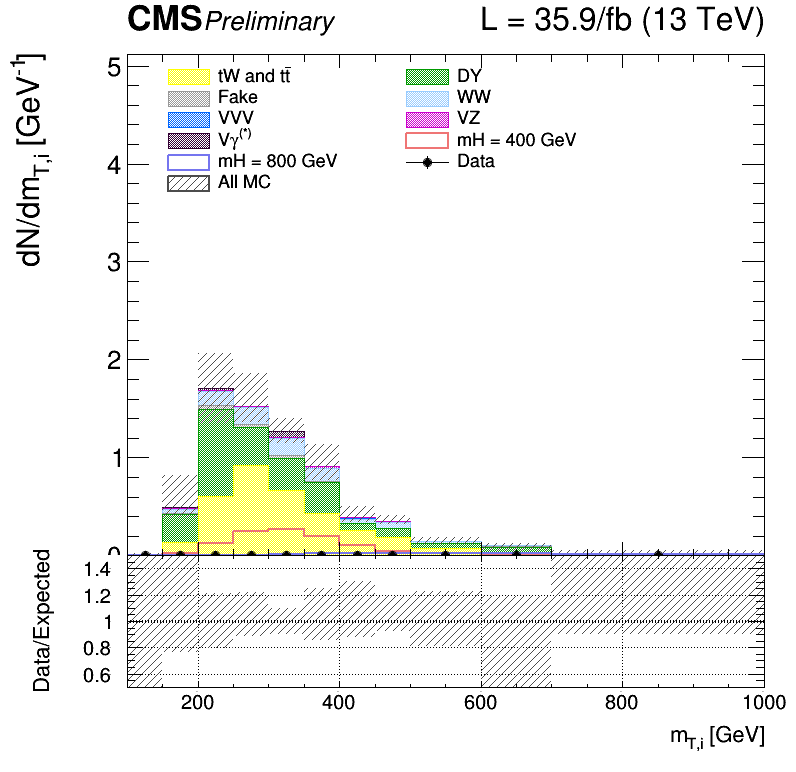
\includegraphics[width=0.45\textwidth]{Figs/SF_SR_Blind/cratio_hwwhm_13TeV_mu_mu_2j_VBF_mTi.png}
}
\subfigure[$m_T^H$]{
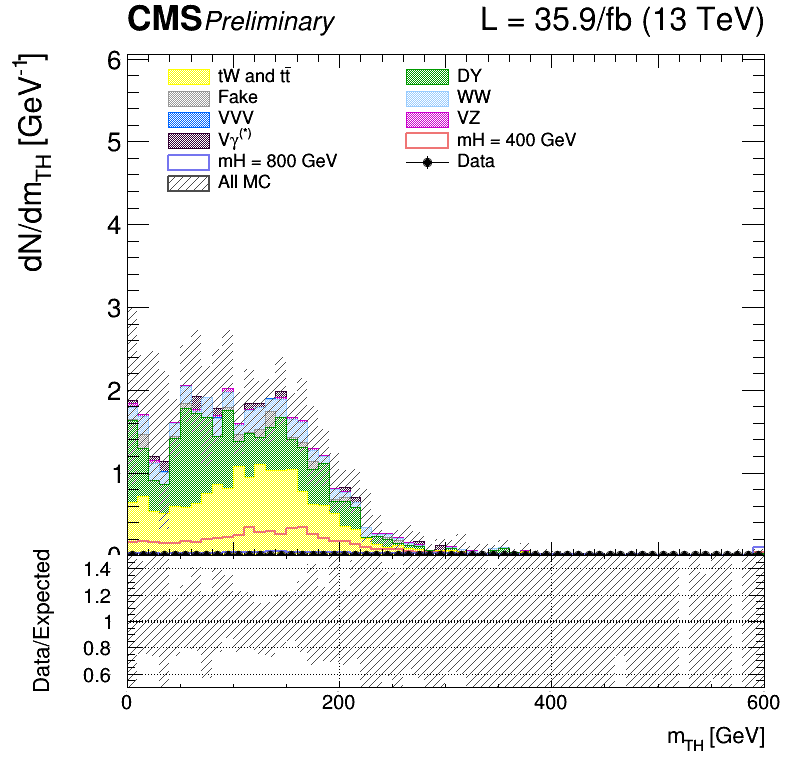
\includegraphics[width=0.45\textwidth]{Figs/SF_SR_Blind/cratio_hwwhm_13TeV_mu_mu_2j_VBF_mth.png}
}
\\
\subfigure[$m_{\ell \ell}$]{
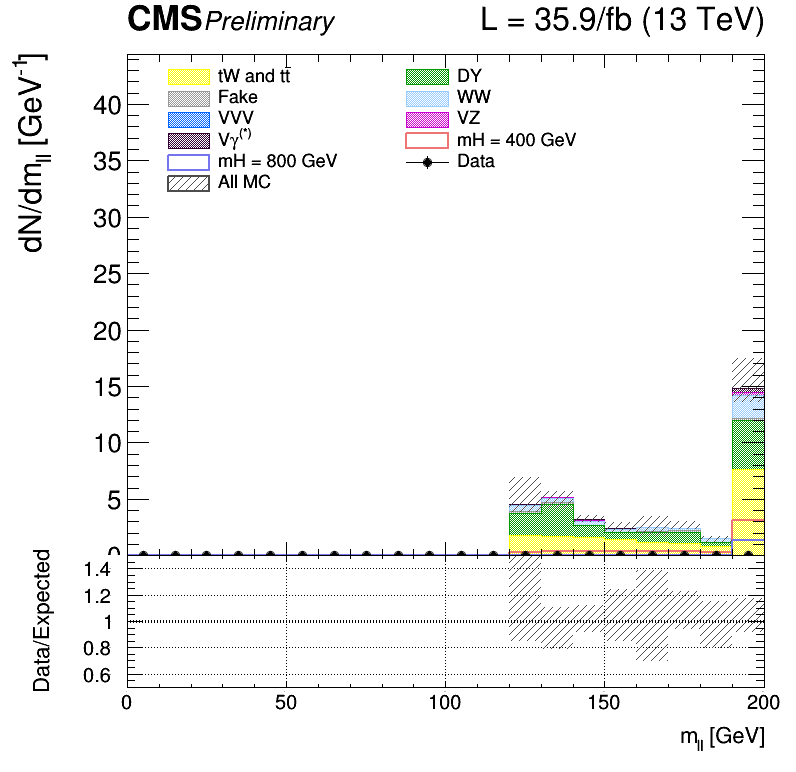
\includegraphics[width=0.45\textwidth]{Figs/SF_SR_Blind/cratio_hwwhm_13TeV_mu_mu_2j_VBF_mll_DY.png}
}
\subfigure[$m_{jj}$]{
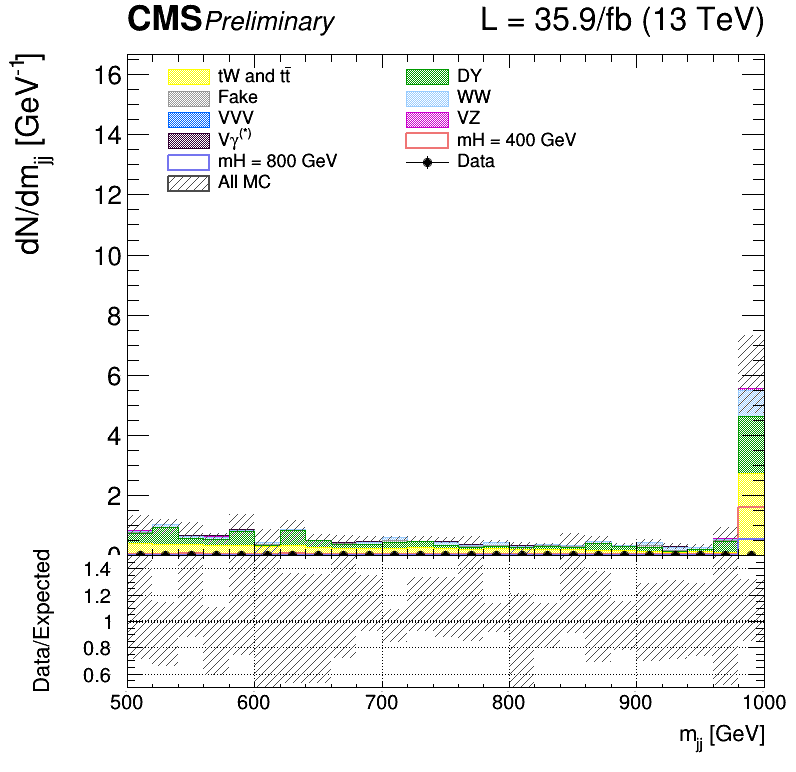
\includegraphics[width=0.45\textwidth]{Figs/SF_SR_Blind/cratio_hwwhm_13TeV_mu_mu_2j_VBF_mjj_DY.png}
}
\caption{Distributions  $m_T^I$, $m_T^I$, $m_T^H$, $m_{\ell \ell}$ and $m_{jj}$ in the signal region $\mu^{\pm} \mu^{\mp}$ case. Two different signal hypothesis corresponding to $m_X = $400 GeV and $m_X = $800 GeV are shown superimposed to the background as a comparison.}
    \label{fig:mti_sigSFmm}
\end{figure}

\subsection{Signal region Unblinding}
The unblinding  $m_T^I$ distribution of the signal regions is shown is Fig. \ref{fig:mti_sigOF_Un} and Fig. \ref{fig:mti_sigOF_Un_log} 

\begin{figure}[htbp]
\centering
\subfigure[ee]{
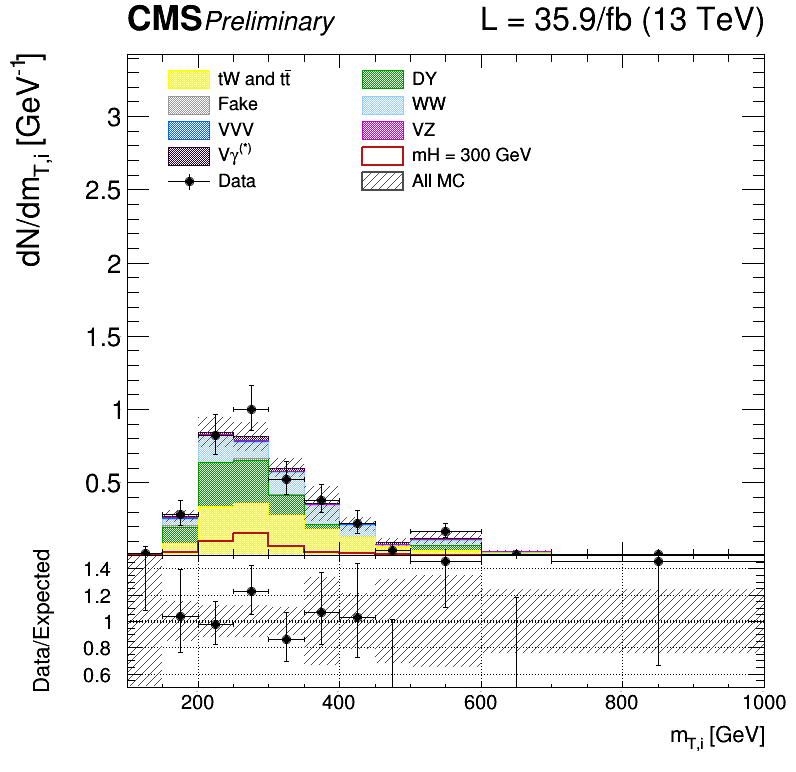
\includegraphics[width=0.45\textwidth]{Figs/unblinding/plot_SR/plotHWWhighMass_SF_ee_postfit_300/cratio_hwwhm_13TeV_sfVBF_ee_mTi.png}
}
\subfigure[mm]{
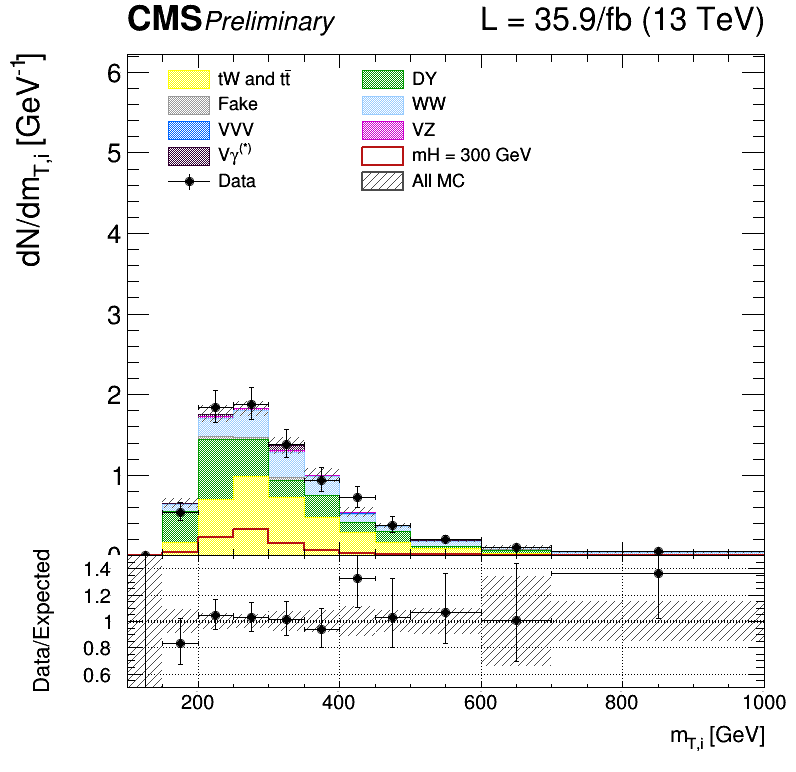
\includegraphics[width=0.45\textwidth]{Figs/unblinding/plot_SR/plotHWWhighMass_SF_mm_postfit_300/cratio_hwwhm_13TeV_sfVBF_mm_mTi.png}
}
\\
\subfigure[ee]{
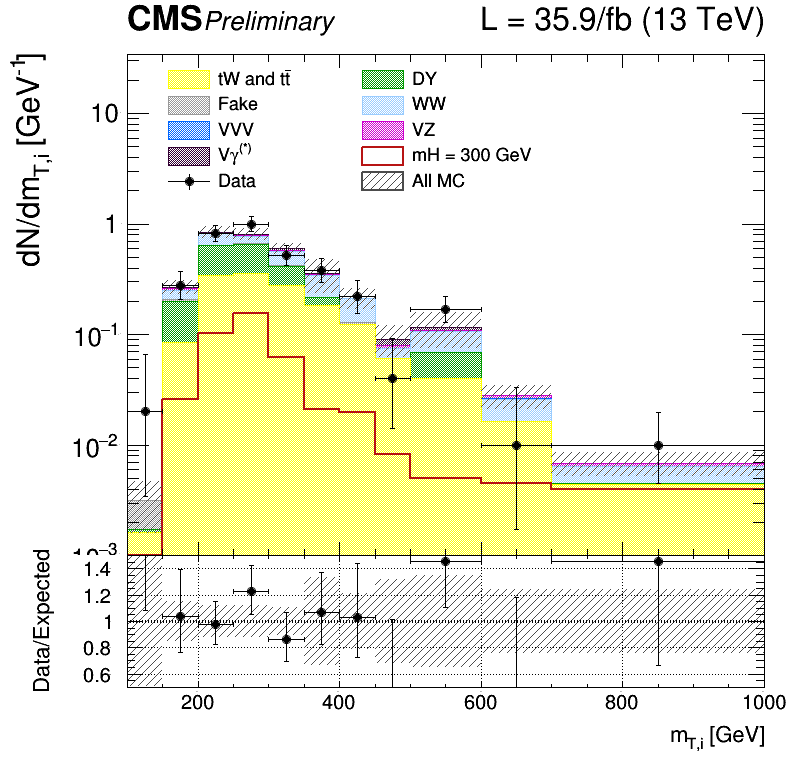
\includegraphics[width=0.45\textwidth]{Figs/unblinding/plot_SR/plotHWWhighMass_SF_ee_postfit_300/log_cratio_hwwhm_13TeV_sfVBF_ee_mTi.png}
}
\subfigure[mm]{
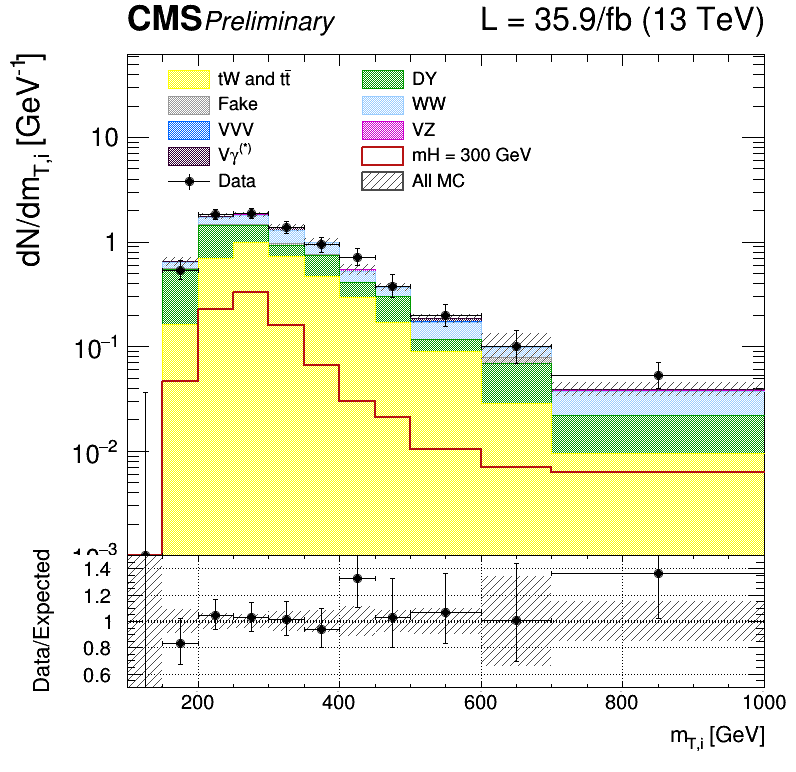
\includegraphics[width=0.45\textwidth]{Figs/unblinding/plot_SR/plotHWWhighMass_SF_mm_postfit_300/log_cratio_hwwhm_13TeV_sfVBF_mm_mTi.png}
}
\caption{Unblinding distributions  $m_T^I$ in the signal region for $ee$ and $\mu \mu$ categories in linear and log scale. The signal hypothesis corresponding to $m_X $ of 300 GeV.}
    \label{fig:mti_sigOF_Un}
\end{figure}




\newpage


\subsection{Drell-Yan control region}
The main background for the SF analysis is the DY. 
A control region has been defined, as close as possible to the signal one to
be used for the normalization of the DY background, separately for electrons
an muons.\\
The control region is defined by the ``WW SF selection'', except for the
$m_{\ell \ell}$ requirement which is changed to 70 GeV $ <m_{\ell \ell} <$ 120
GeV to include the Z boson.

The Missing Transverse Energy ditribution in the data shows discrepancies respect to Monte Carlo simulation  in ee and $\mu \mu$ Drell-Yan control regions. A correction is applied reweighting all the simulated samples with a weight per event which depends on the MET value. 
The weight is evaluated as the ratio between data, one subtracted all backgraounds except the DY, and the Drell-Yan itself, in each bins of the distribution, separately for ee and $\mu \mu$ categories. The weight is assumed to be linear as function of the MET value.\\
This kind of reweighting allows to correct for shape differences between data and MC, , Fig. \ref{fig:dy_met}.


The control plots for several variables in a Drell-Yan enriched phase space
for the ee and $\mu \mu$ are shown in Figs.~\ref{fig:mll_sigSF_CR_DY_ee} for
the dielectron case and Figs.~\ref{fig:mll_sigSF_CR_DY_mm} for the dimuon
case. In general there is a good agreement betwen data and MC.

\newpage

\begin{figure}[htbp]
\centering
\subfigure[ee before the reweight]{
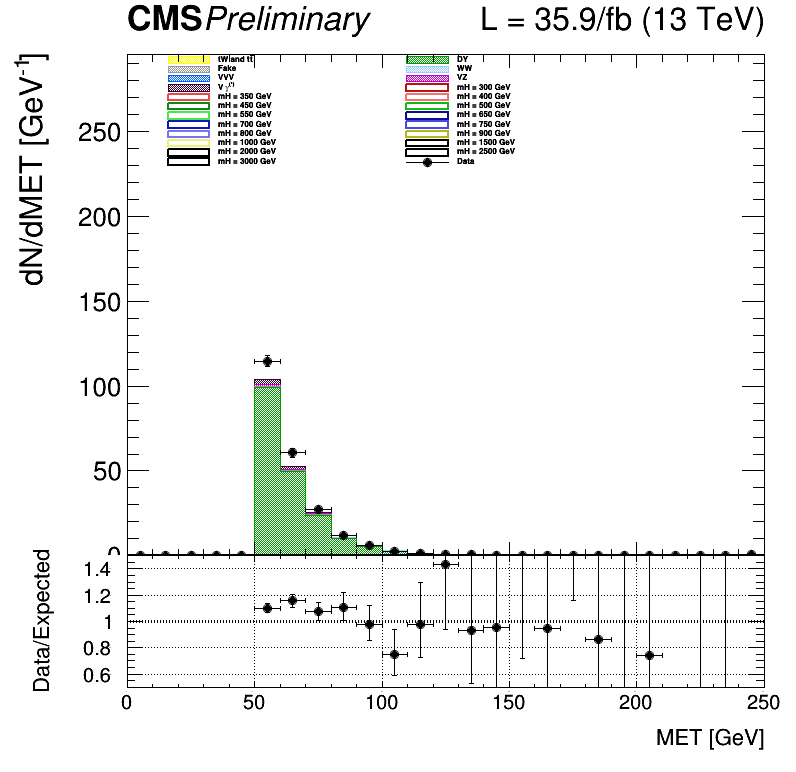
\includegraphics[width=0.45\textwidth]{Figs/METrw/cratio_hww2l2v_13TeV_dy_e_e_2j_VBF_metPfType1.png}
}
\subfigure[$\mu \mu$  before the reweight]{
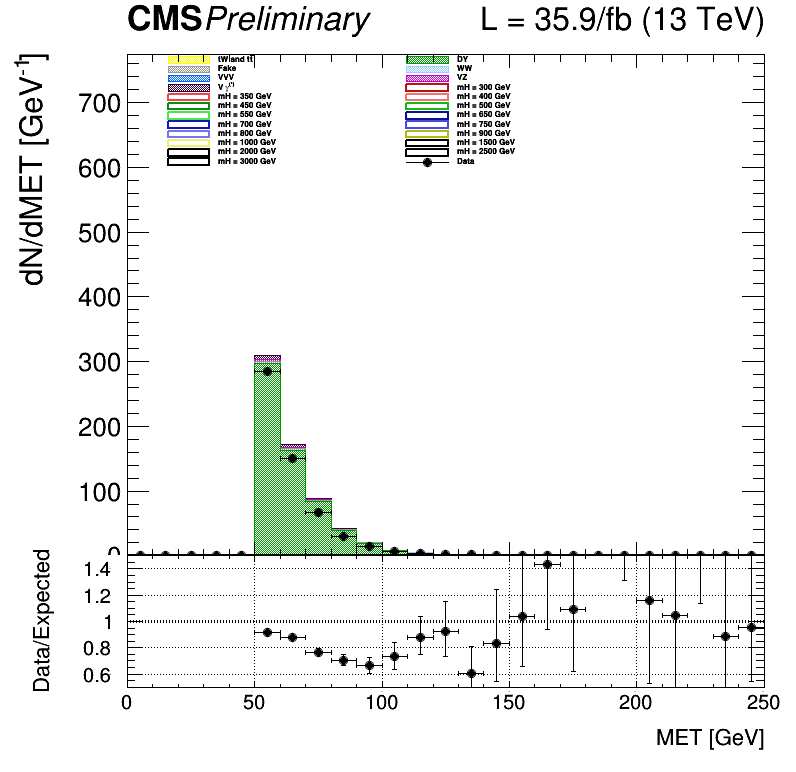
\includegraphics[width=0.45\textwidth]{Figs/METrw/cratio_hww2l2v_13TeV_dy_mu_mu_2j_VBF_metPfType1.png}
}                                              

\subfigure[ee  after the reweight]{
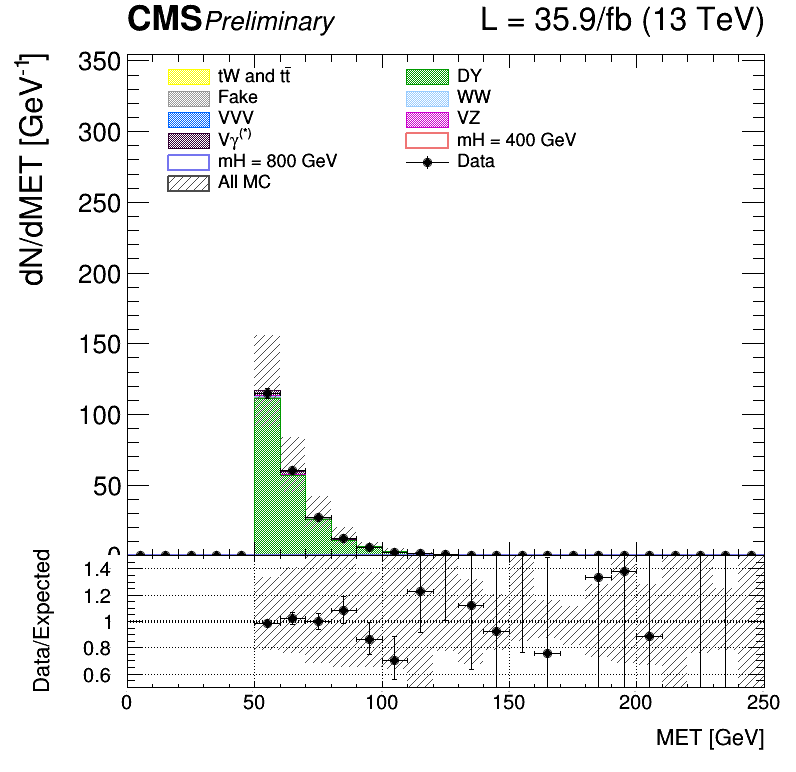
\includegraphics[width=0.45\textwidth]{Figs/SF_CR_Blind/cratio_hww2l2v_13TeV_dy_e_e_2j_VBF_metPfType1.png}
}
\subfigure[$\mu \mu$  after the reweight]{
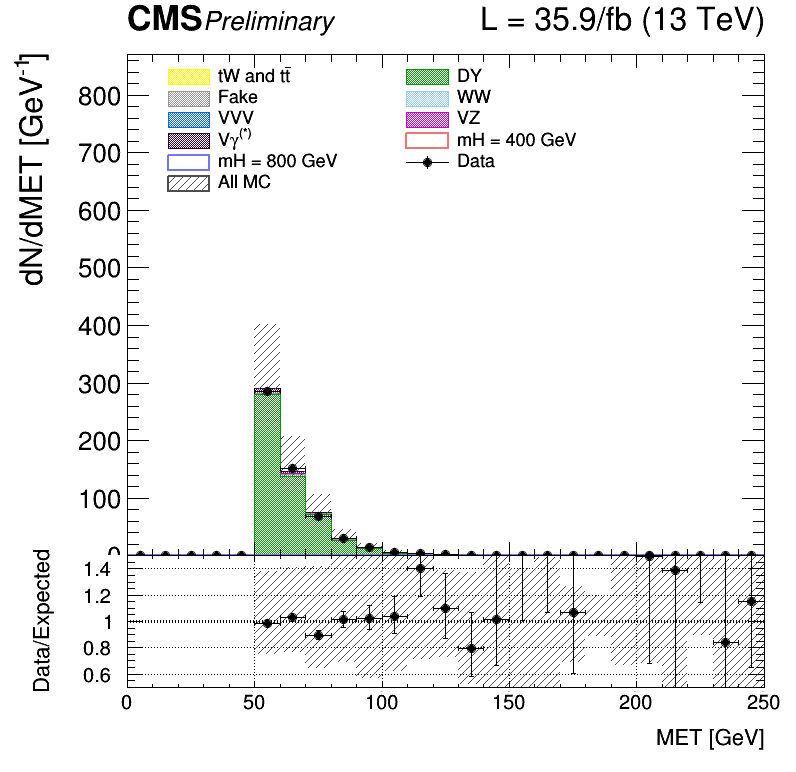
\includegraphics[width=0.45\textwidth]{Figs/SF_CR_Blind/cratio_hww2l2v_13TeV_dy_mu_mu_2j_VBF_metPfType1.png}
}                   

\caption{MET control plots for Drell-Yan fot ee categories in \textit{a} and for $\mu \mu$ in \textit{b} before the reweight. In \textit{c} and  \textit{d} the same 
distribution after the correction.}
    \label{fig:dy_met}                                             

\end{figure}\\




\newpage

\begin{figure}[htbp]
\centering
\subfigure[$m_T^I$]{
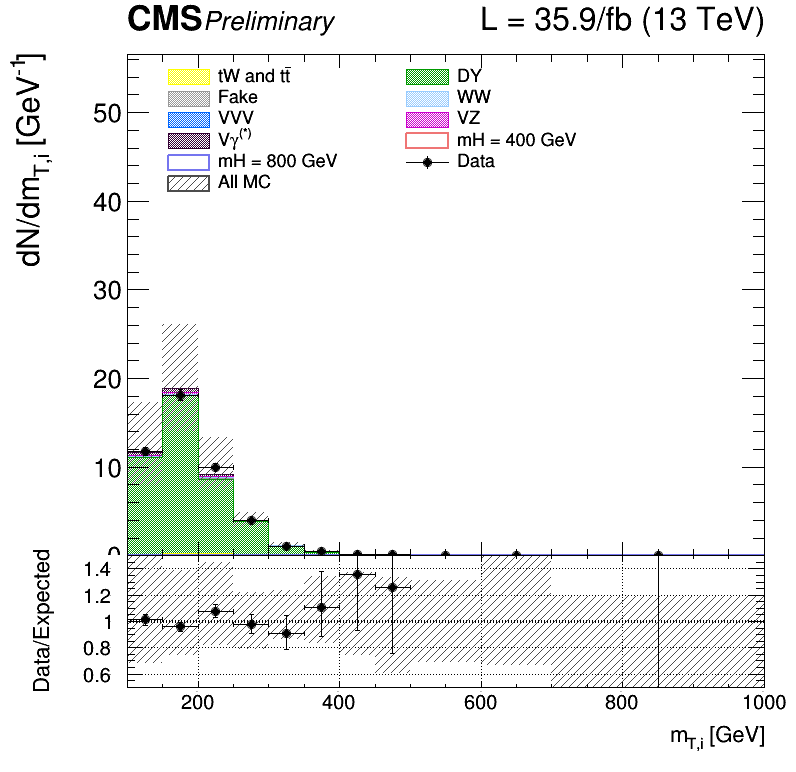
\includegraphics[width=0.45\textwidth]{Figs/SF_CR_Blind/cratio_hww2l2v_13TeV_dy_e_e_2j_VBF_mTi.png}
}
\subfigure[$m_T^H$]{
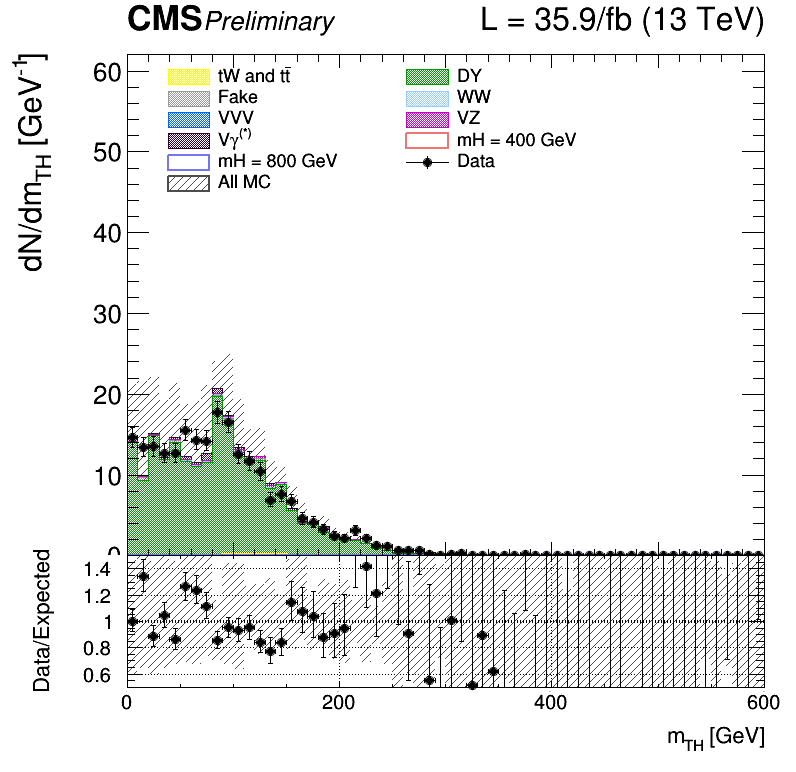
\includegraphics[width=0.45\textwidth]{Figs/SF_CR_Blind/cratio_hww2l2v_13TeV_dy_e_e_2j_VBF_mth.png}
}                                              
\\                                             
\subfigure[$m_{jj}$]{                             
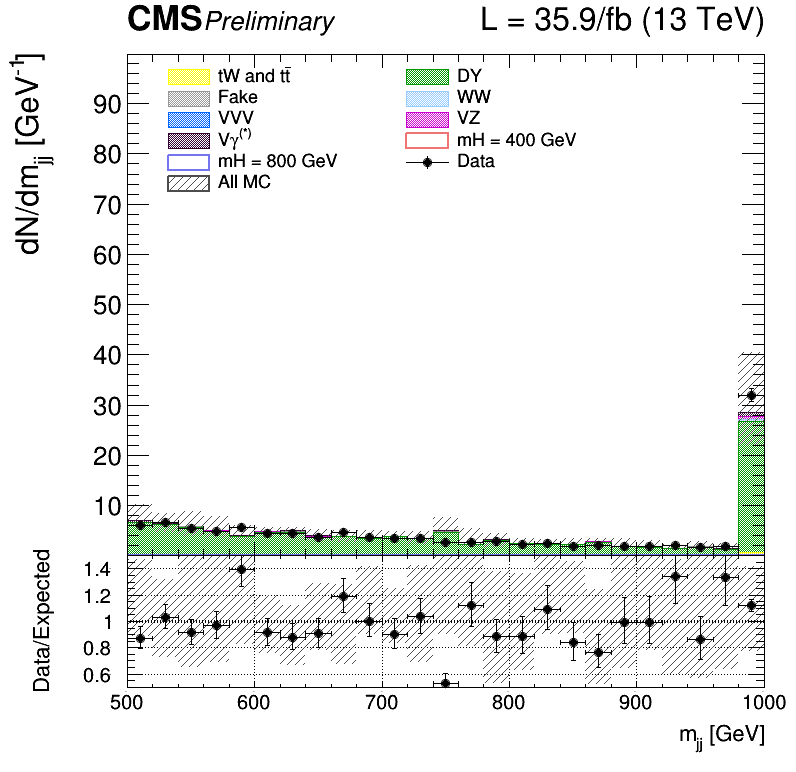
\includegraphics[width=0.45\textwidth]{Figs/SF_CR_Blind/cratio_hww2l2v_13TeV_dy_e_e_2j_VBF_mjj_DY.png}
}                                              
\subfigure[$m_{\ell \ell}$]{                               
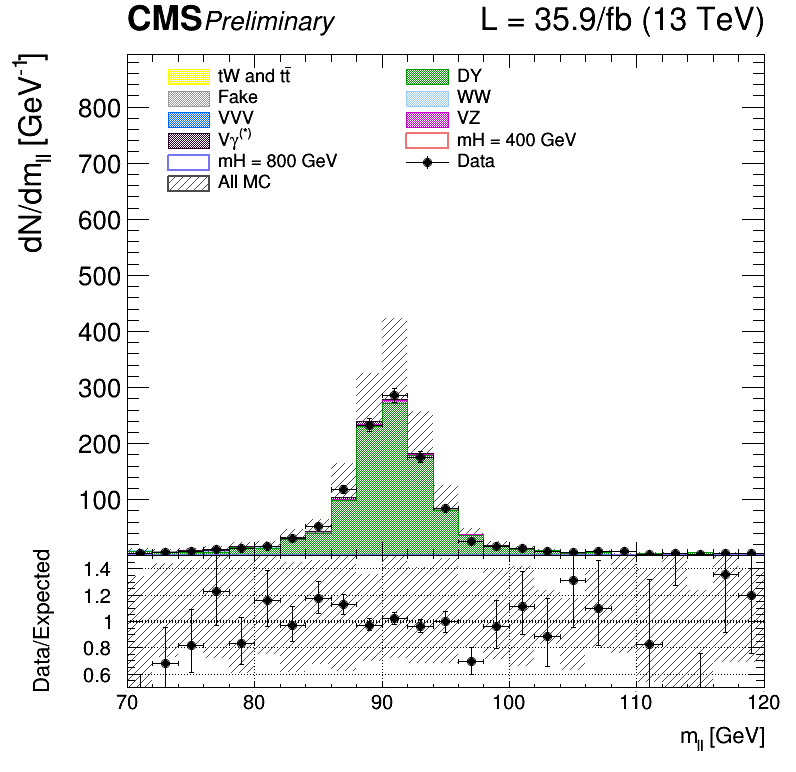
\includegraphics[width=0.45\textwidth]{Figs/SF_CR_Blind/cratio_hww2l2v_13TeV_dy_e_e_2j_VBF_mll.png}
}\\

\subfigure[$p_T$ leading lepton]{                             
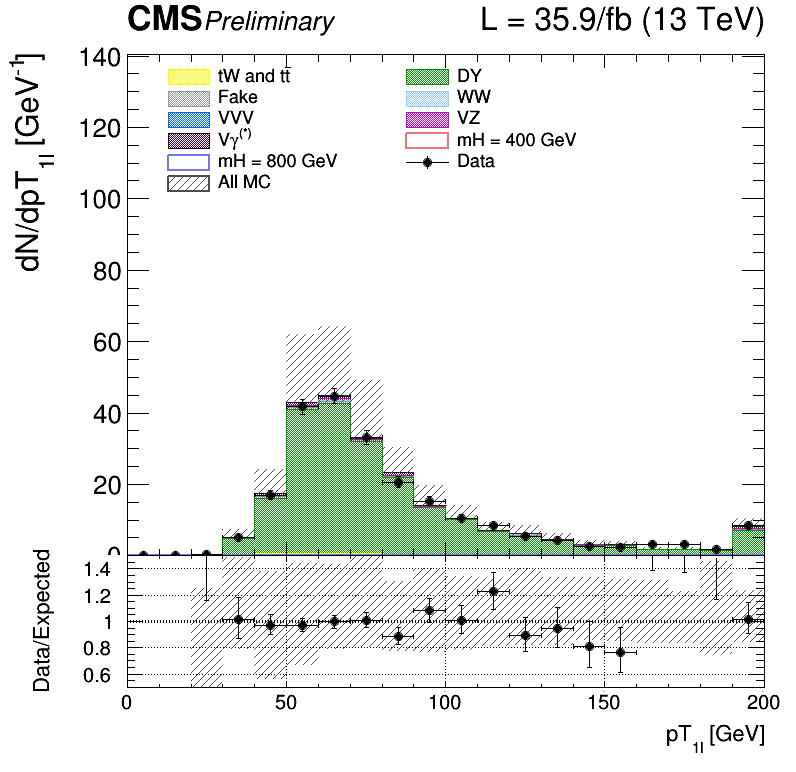
\includegraphics[width=0.45\textwidth]{Figs/SF_CR_Blind/cratio_hww2l2v_13TeV_dy_e_e_2j_VBF_std_vector_lepton_pt[0].png}
}                                              
\subfigure[$p_T^{\ell \ell}$]{                               
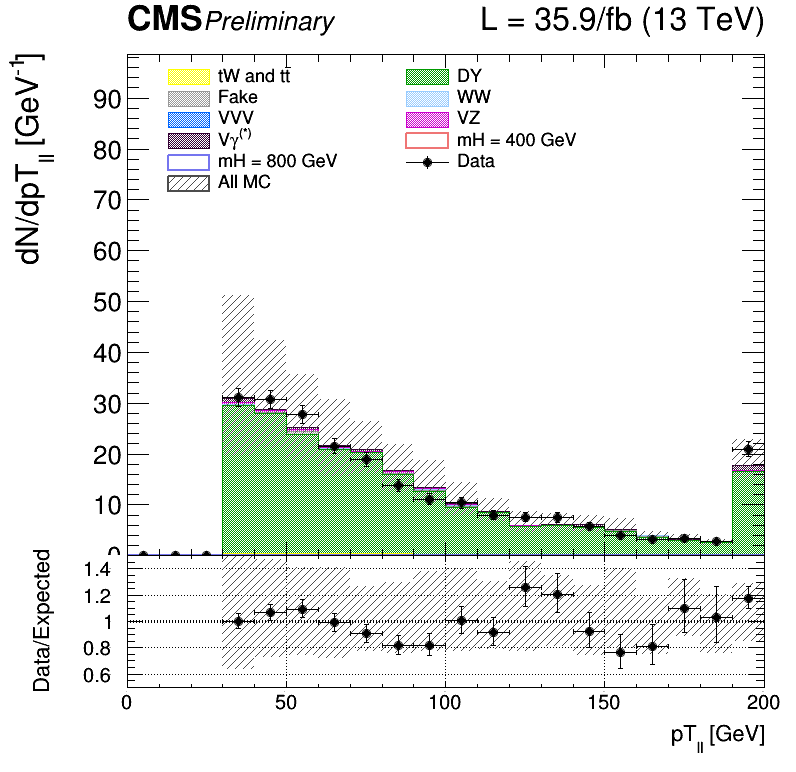
\includegraphics[width=0.45\textwidth]{Figs/SF_CR_Blind/cratio_hww2l2v_13TeV_dy_e_e_2j_VBF_ptll.png}
}\\

\caption{Control plots for several variables in a Drell-Yan enriched phase space for ee.}
    \label{fig:mll_sig}
\end{figure}

\newpage

\begin{figure}[htbp]
\centering
\subfigure[$m_T^I$]{
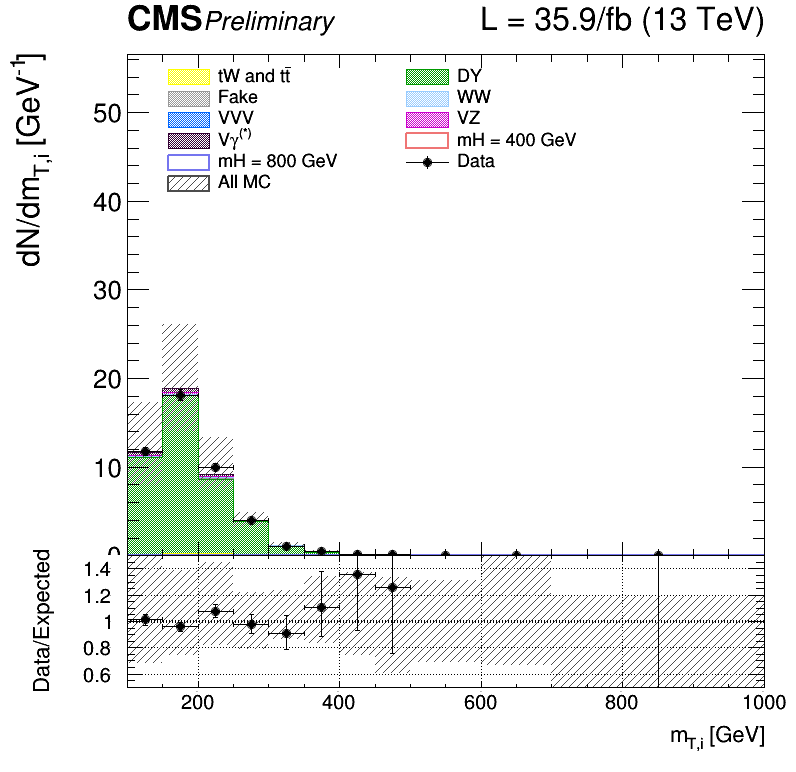
\includegraphics[width=0.45\textwidth]{Figs/SF_CR_Blind/cratio_hww2l2v_13TeV_dy_e_e_2j_VBF_mTi.png}
}
\subfigure[$m_T^H$]{
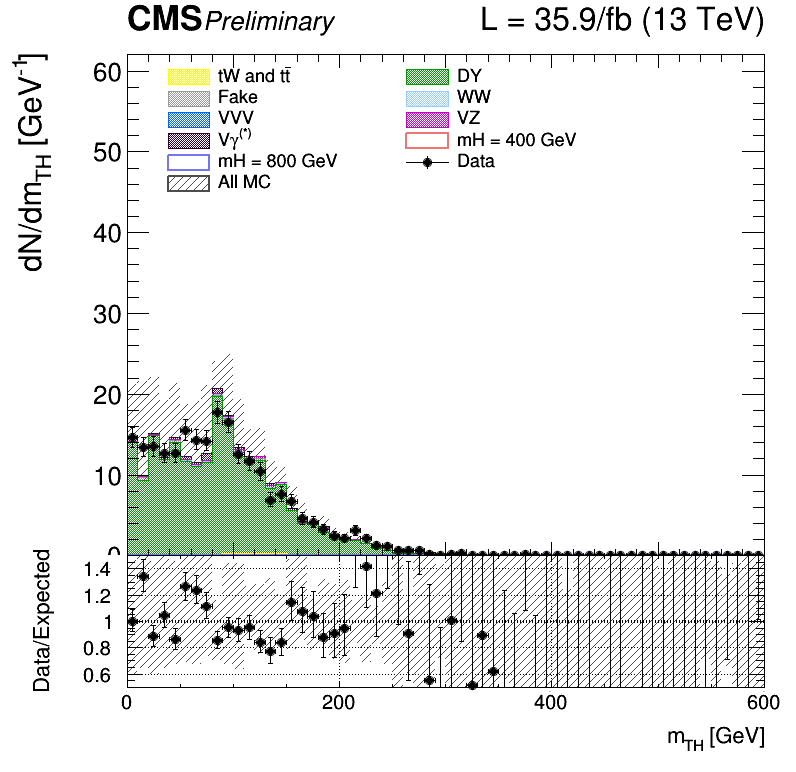
\includegraphics[width=0.45\textwidth]{Figs/SF_CR_Blind/cratio_hww2l2v_13TeV_dy_e_e_2j_VBF_mth.png}
}                                              
\\                                             
\subfigure[$m_{jj}$]{                             
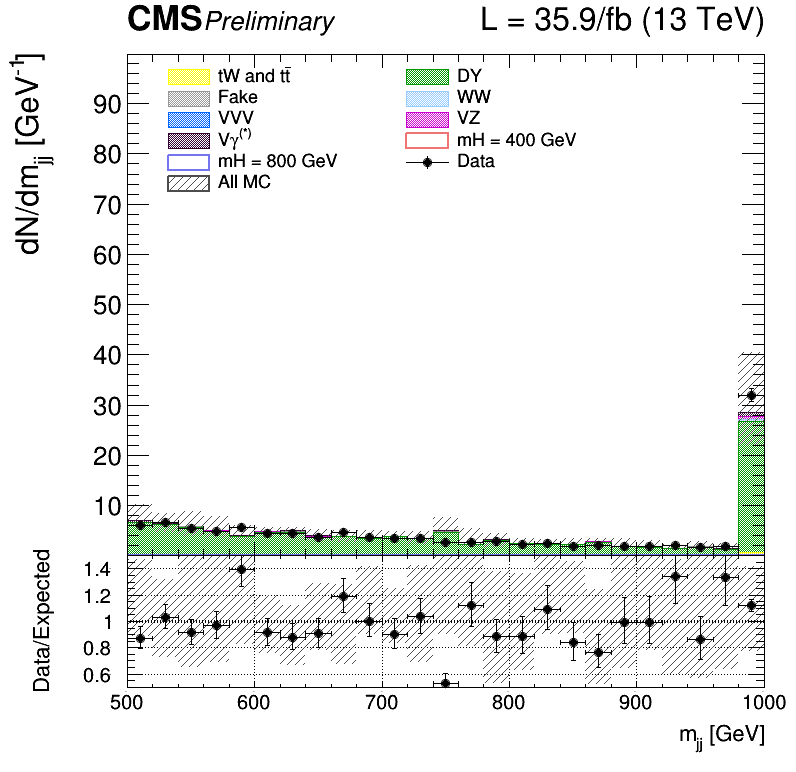
\includegraphics[width=0.45\textwidth]{Figs/SF_CR_Blind/cratio_hww2l2v_13TeV_dy_e_e_2j_VBF_mjj_DY.png}
}                                              
\subfigure[$m_{\ell \ell}$]{                               
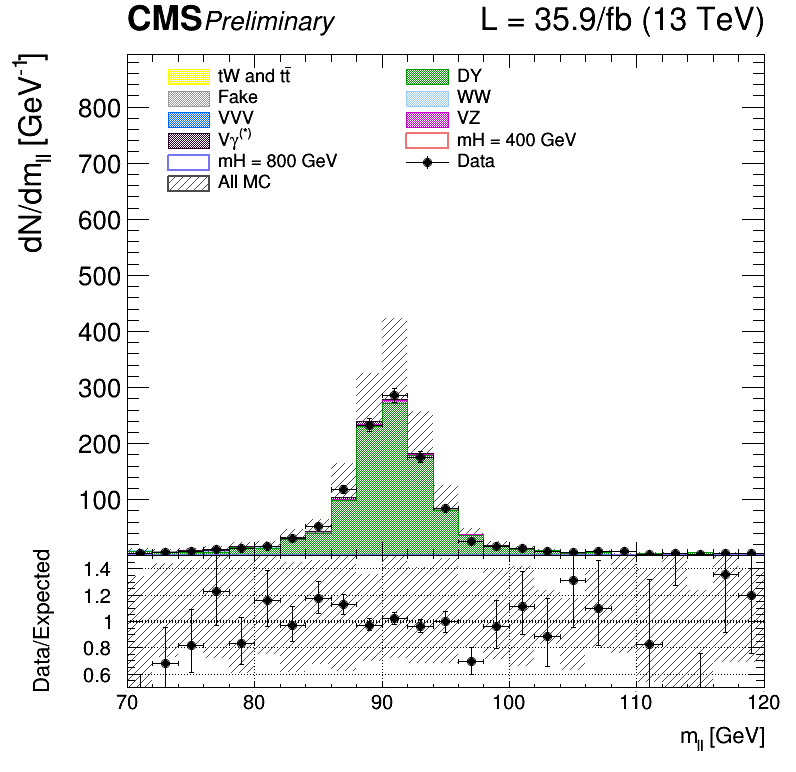
\includegraphics[width=0.45\textwidth]{Figs/SF_CR_Blind/cratio_hww2l2v_13TeV_dy_e_e_2j_VBF_mll.png}
}\\

\subfigure[$p_T$ leading lepton]{                             
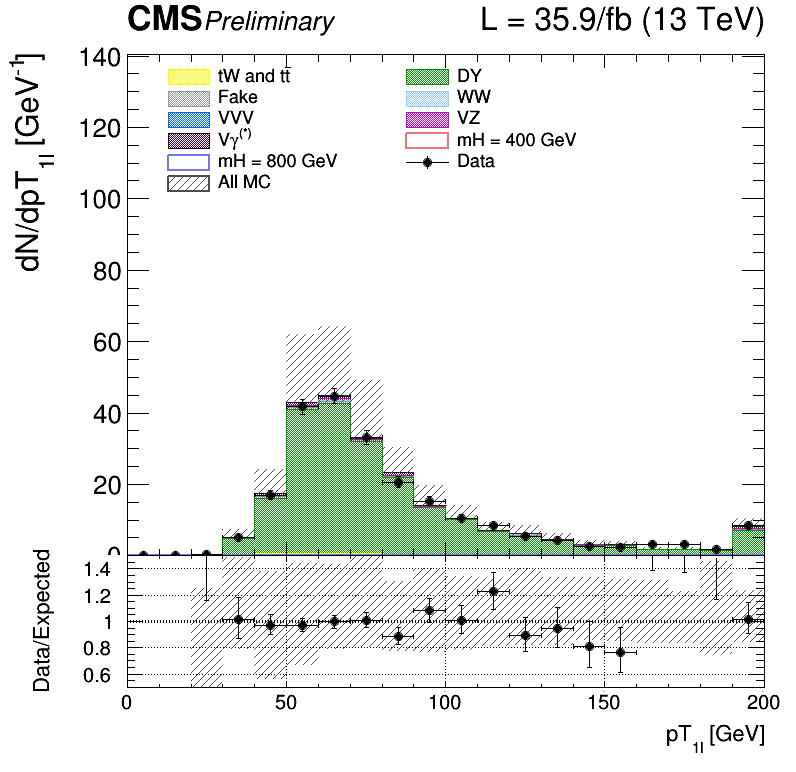
\includegraphics[width=0.45\textwidth]{Figs/SF_CR_Blind/cratio_hww2l2v_13TeV_dy_e_e_2j_VBF_std_vector_lepton_pt[0].png}
}                                              
\subfigure[$p_T^{\ell \ell}$]{                               
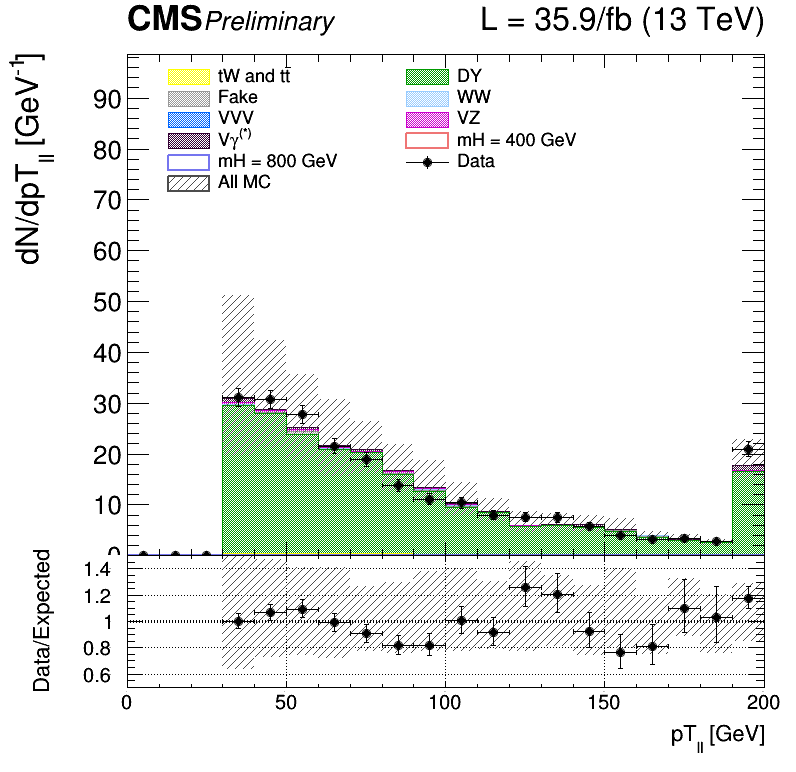
\includegraphics[width=0.45\textwidth]{Figs/SF_CR_Blind/cratio_hww2l2v_13TeV_dy_e_e_2j_VBF_ptll.png}
}\\

\caption{Control plots for several variables in a Drell-Yan enriched phase space for ee.}
    \label{fig:mll_sigSF_CR_DY_ee}
\end{figure}


\newpage

\begin{figure}[h]
\centering
\subfigure[$m_T^I$]{
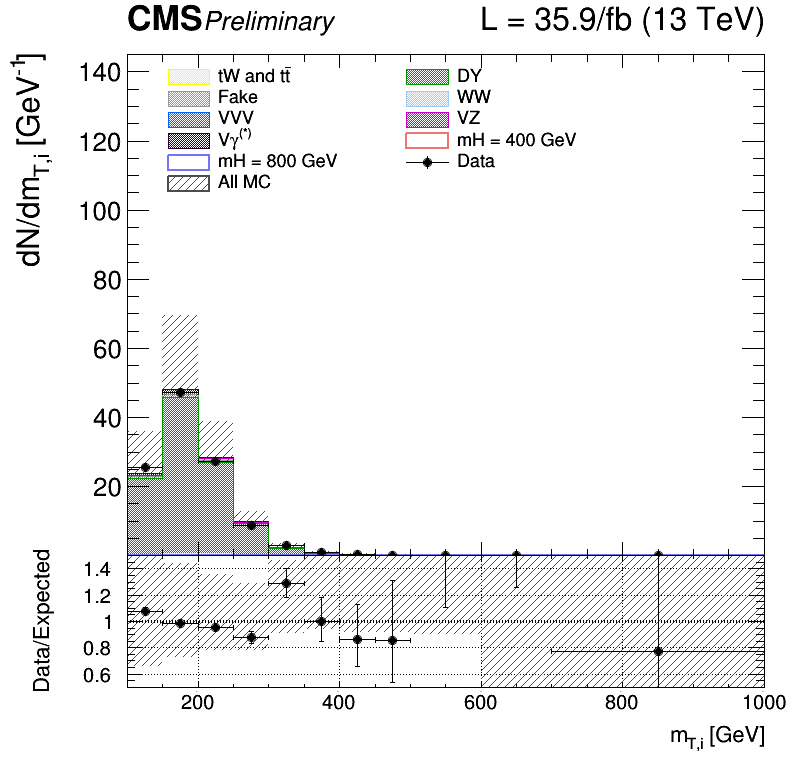
\includegraphics[width=0.45\textwidth]{Figs/SF_CR_Blind/cratio_hww2l2v_13TeV_dy_mu_mu_2j_VBF_mTi.png}
}
\subfigure[$m_T^H$]{
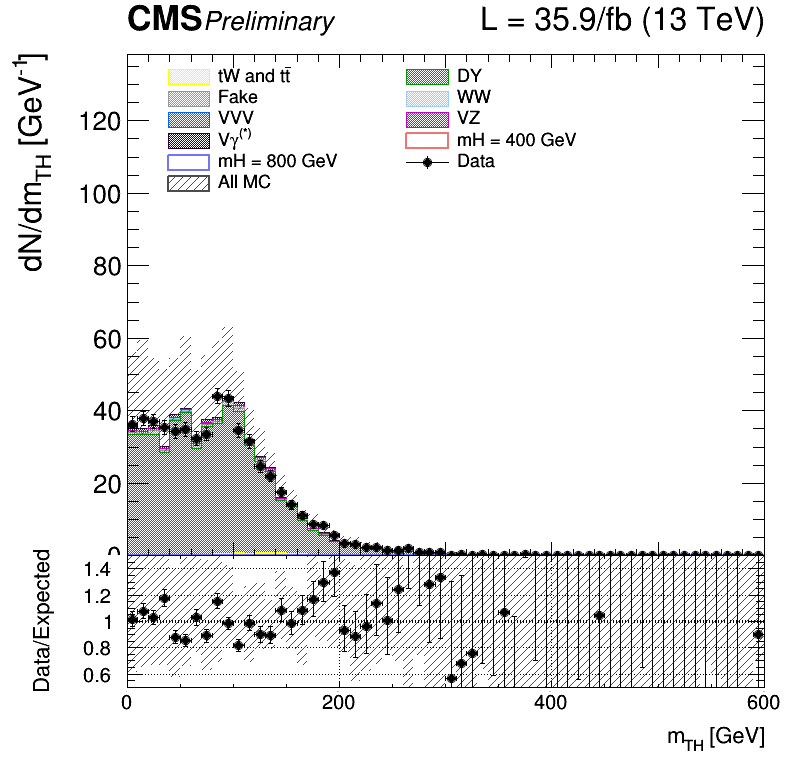
\includegraphics[width=0.45\textwidth]{Figs/SF_CR_Blind/cratio_hww2l2v_13TeV_dy_mu_mu_2j_VBF_mth.png}
}                                              
\\                                             
\subfigure[$m_{jj}$]{                             
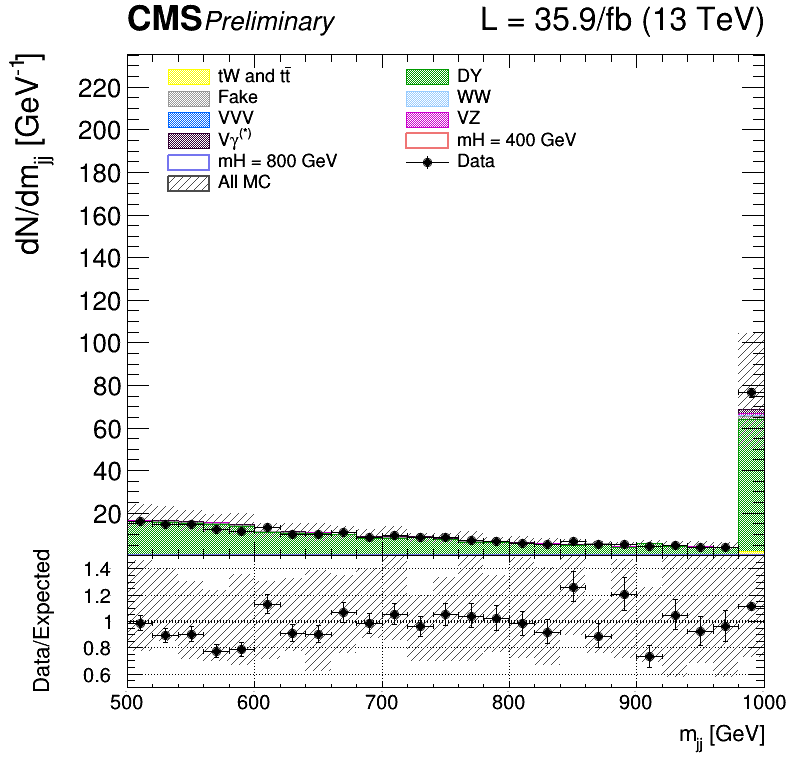
\includegraphics[width=0.45\textwidth]{Figs/SF_CR_Blind/cratio_hww2l2v_13TeV_dy_mu_mu_2j_VBF_mjj_DY.png}
}                                              
\subfigure[$m_{\ell \ell}$]{                               
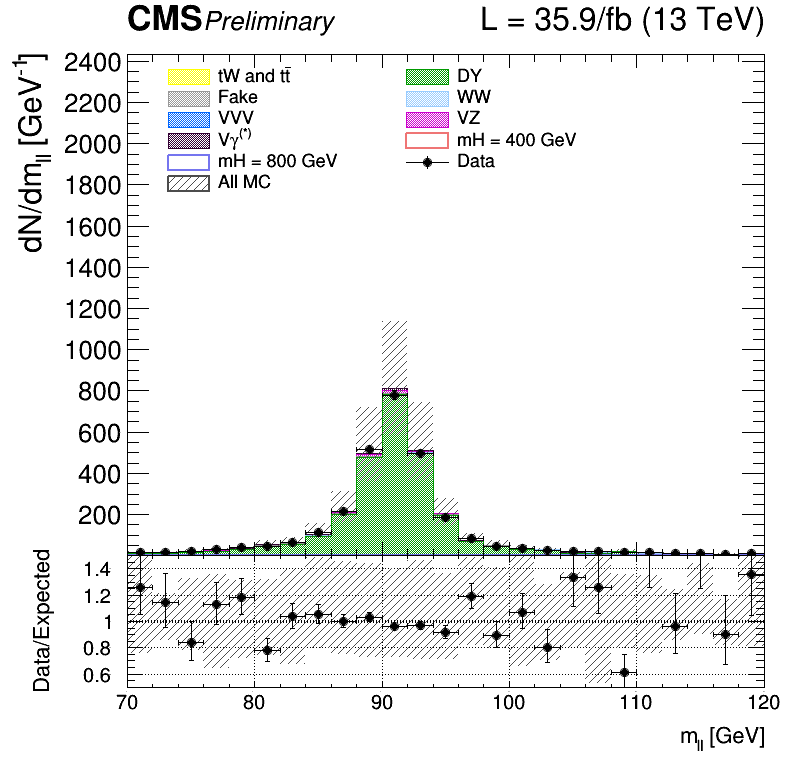
\includegraphics[width=0.45\textwidth]{Figs/SF_CR_Blind/cratio_hww2l2v_13TeV_dy_mu_mu_2j_VBF_mll.png}
}\\

\subfigure[$p_T$ leading lepton]{                             
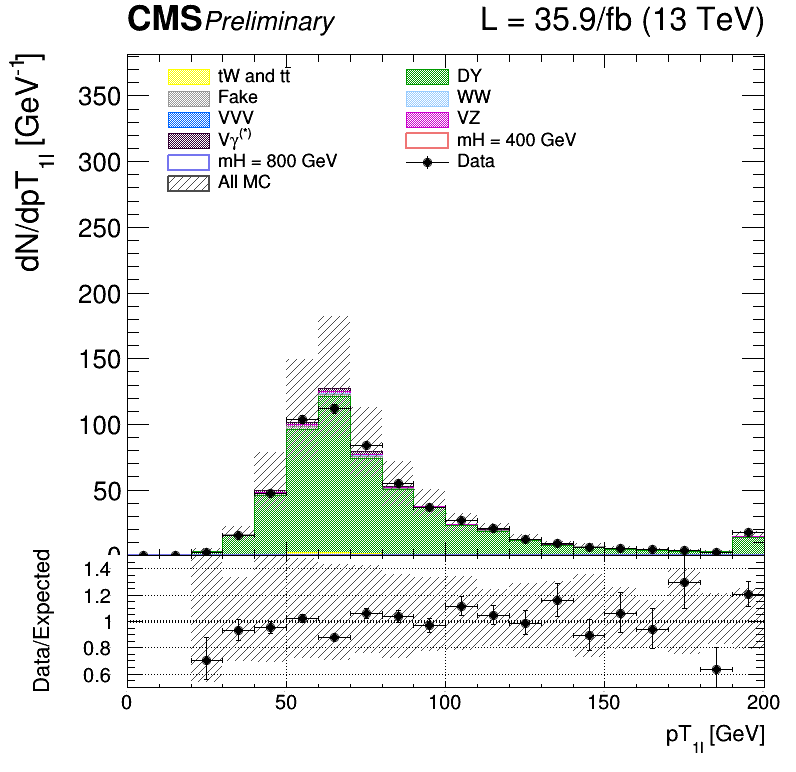
\includegraphics[width=0.45\textwidth]{Figs/SF_CR_Blind/cratio_hww2l2v_13TeV_dy_mu_mu_2j_VBF_std_vector_lepton_pt[0].png}
}                                              
\subfigure[$p_T^{\ell \ell}$]{                               
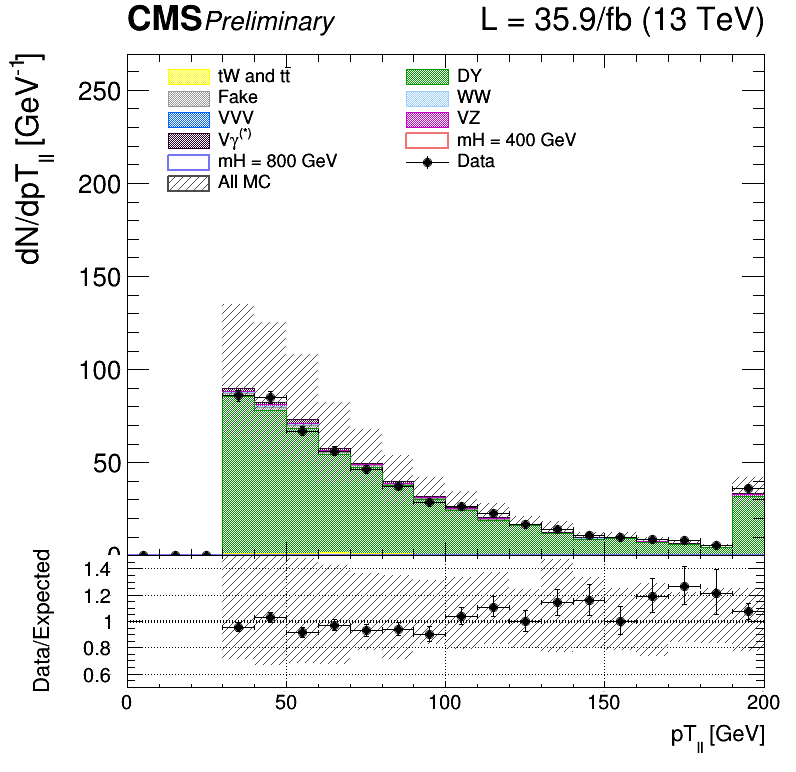
\includegraphics[width=0.45\textwidth]{Figs/SF_CR_Blind/cratio_hww2l2v_13TeV_dy_mu_mu_2j_VBF_ptll.png}
}\\

\caption{Control plots for several variables in a Drell-Yan enriched phase space for $\mu \mu$.}
    \label{fig:mll_sigSF_CR_DY_mm}
\end{figure}

\newpage
\clearpage
\subsection{Top control region}
A top-enriched control region is defined to normalize the top backgrouns,
separately for electrons and muons.
The ``WW SF selection'' is required with the inversion of the b-tagging
requirement, i.e. the two jets are both requested to be b-tagged according to
cMVAv2 loose WP.:

The control plots for several variables in a top enriched phase space for events are shown in
the Figs.~\ref{fig:mll_sigSF_CR_top_ee} for the dielectron case and
\ref{fig:mll_sigSF_CR_top_mm} for the dimuon case. Good agreement is observed
between data and MC.


\begin{figure}[htbp]
\centering
\subfigure[$m_T^I$]{
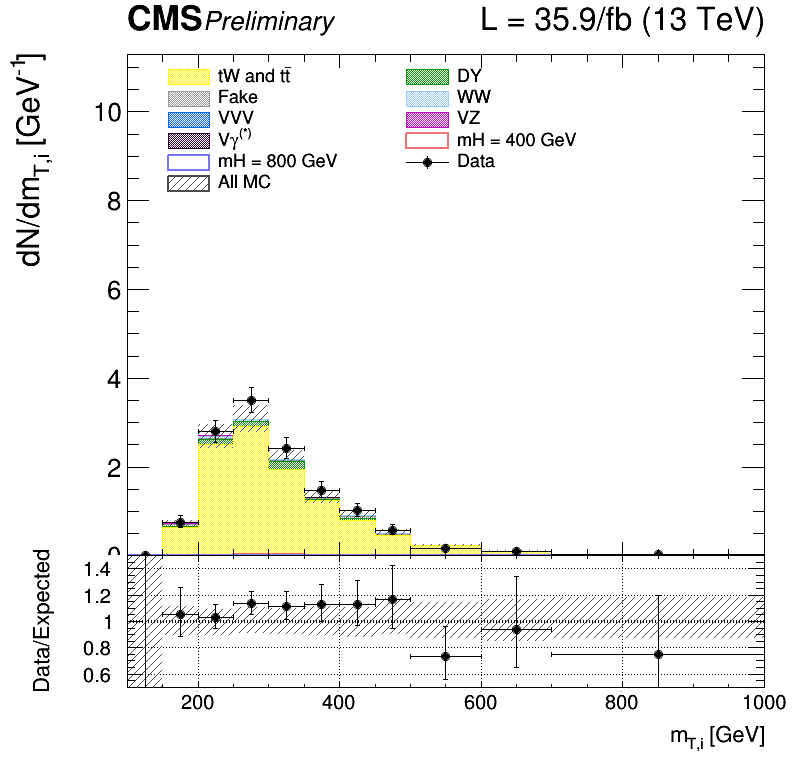
\includegraphics[width=0.45\textwidth]{Figs/SF_CR_Blind/cratio_hww2l2v_13TeV_top_e_e_2j_VBF_mTi.png}
}
\subfigure[$m_T^H$]{
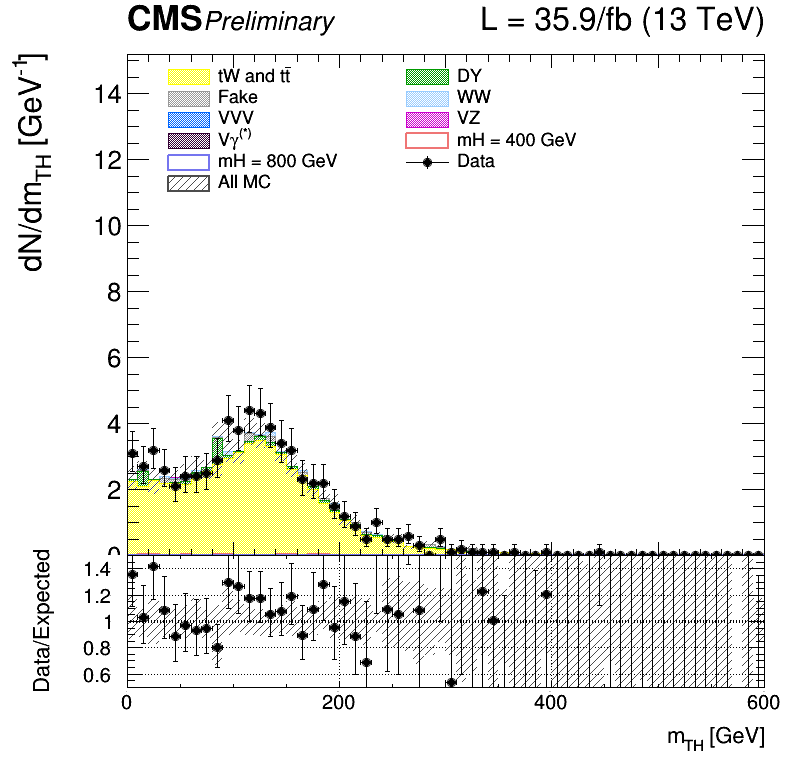
\includegraphics[width=0.45\textwidth]{Figs/SF_CR_Blind/cratio_hww2l2v_13TeV_top_e_e_2j_VBF_mth.png}
}                                              
\\                                             
\subfigure[$m_{jj}$]{                             
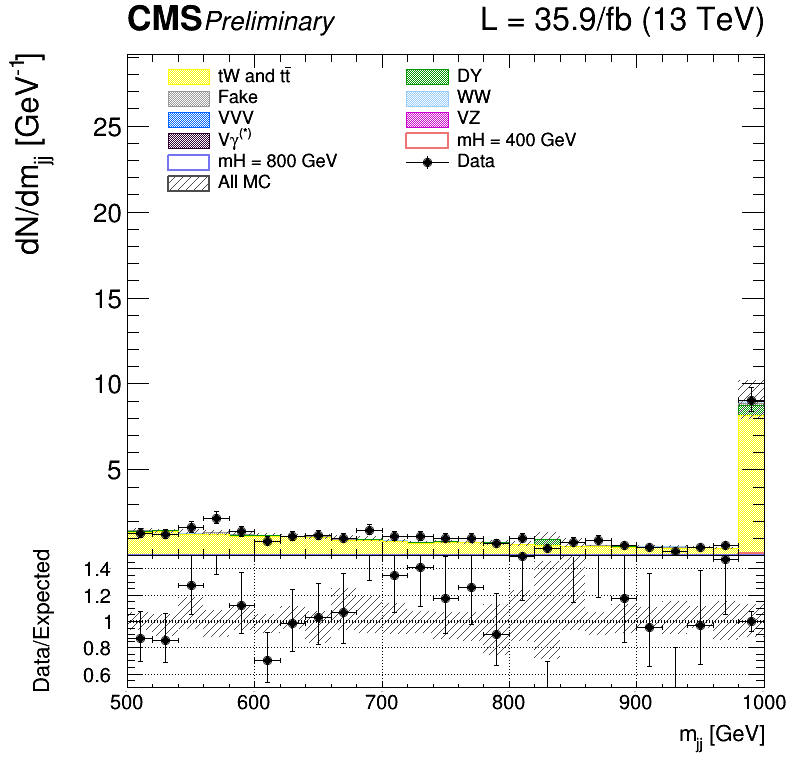
\includegraphics[width=0.45\textwidth]{Figs/SF_CR_Blind/cratio_hww2l2v_13TeV_top_e_e_2j_VBF_mjj_DY.png}
}                                              
\subfigure[$m_{\ell \ell}$]{                               
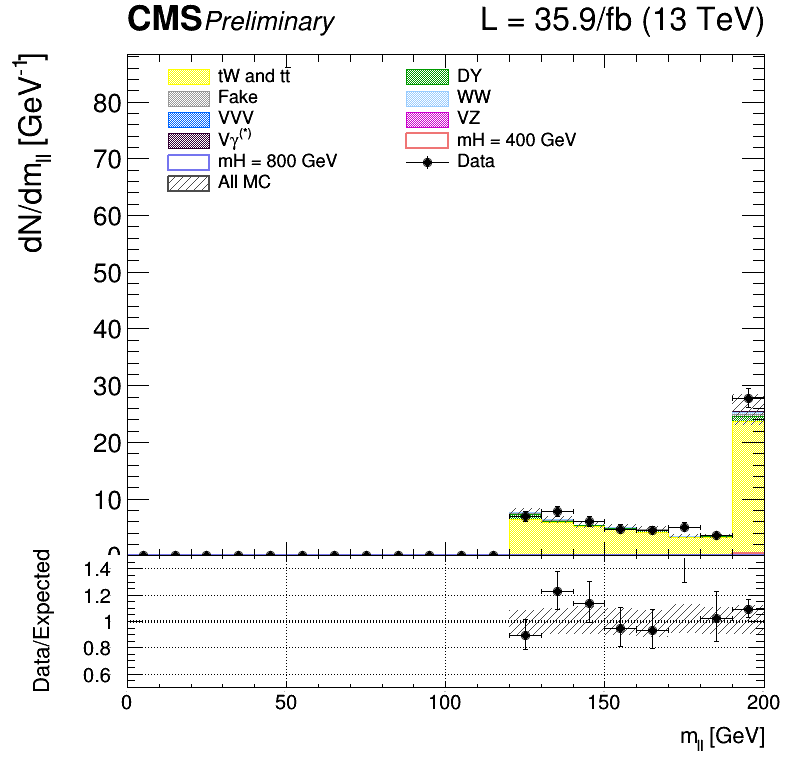
\includegraphics[width=0.45\textwidth]{Figs/SF_CR_Blind/cratio_hww2l2v_13TeV_top_e_e_2j_VBF_mll_DY.png}
}\\

\subfigure[$p_T$ leading lepton]{                             
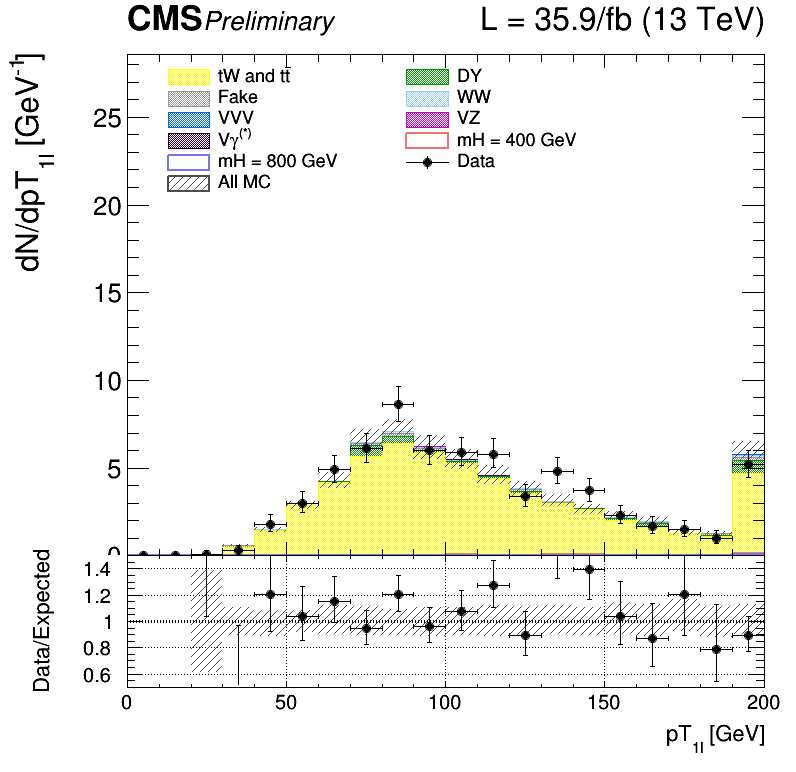
\includegraphics[width=0.45\textwidth]{Figs/SF_CR_Blind/cratio_hww2l2v_13TeV_top_e_e_2j_VBF_std_vector_lepton_pt[0].png}
}                                              
\subfigure[$p_T^{\ell \ell}$]{                               
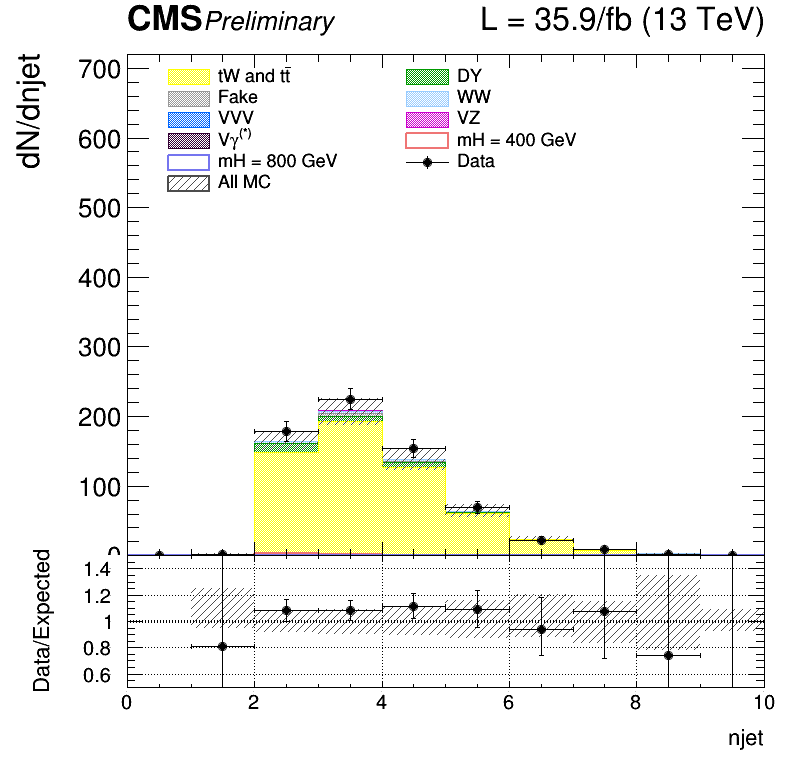
\includegraphics[width=0.45\textwidth]{Figs/SF_CR_Blind/cratio_hww2l2v_13TeV_top_e_e_2j_VBF_njet.png}
}\\

\caption{Control plots for several variables in a Top enriched phase space for ee.}
    \label{fig:mll_sigSF_CR_top_ee}
\end{figure}




\begin{figure}[htbp]
\centering
\subfigure[$m_T^I$]{
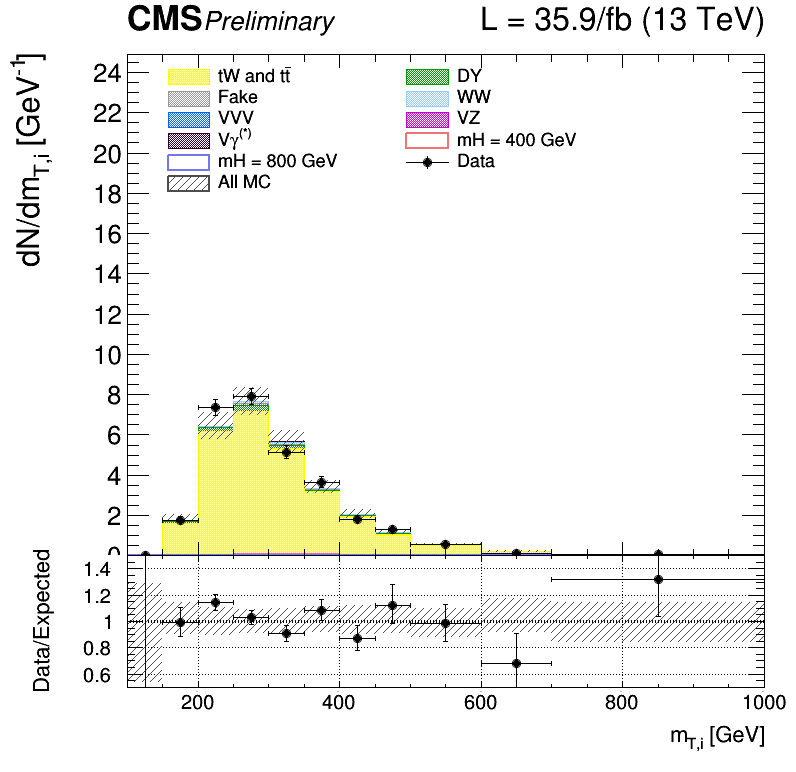
\includegraphics[width=0.45\textwidth]{Figs/SF_CR_Blind/cratio_hww2l2v_13TeV_top_mu_mu_2j_VBF_mTi.png}
}
\subfigure[$m_T^H$]{
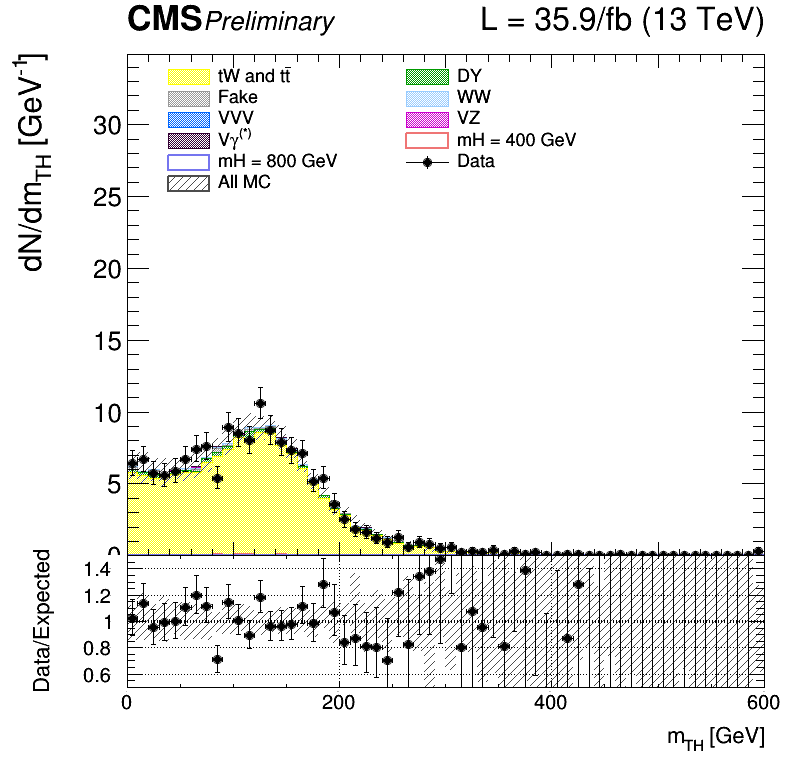
\includegraphics[width=0.45\textwidth]{Figs/SF_CR_Blind/cratio_hww2l2v_13TeV_top_mu_mu_2j_VBF_mth.png}
}                                              
\\                                             
\subfigure[$m_{jj}$]{                             
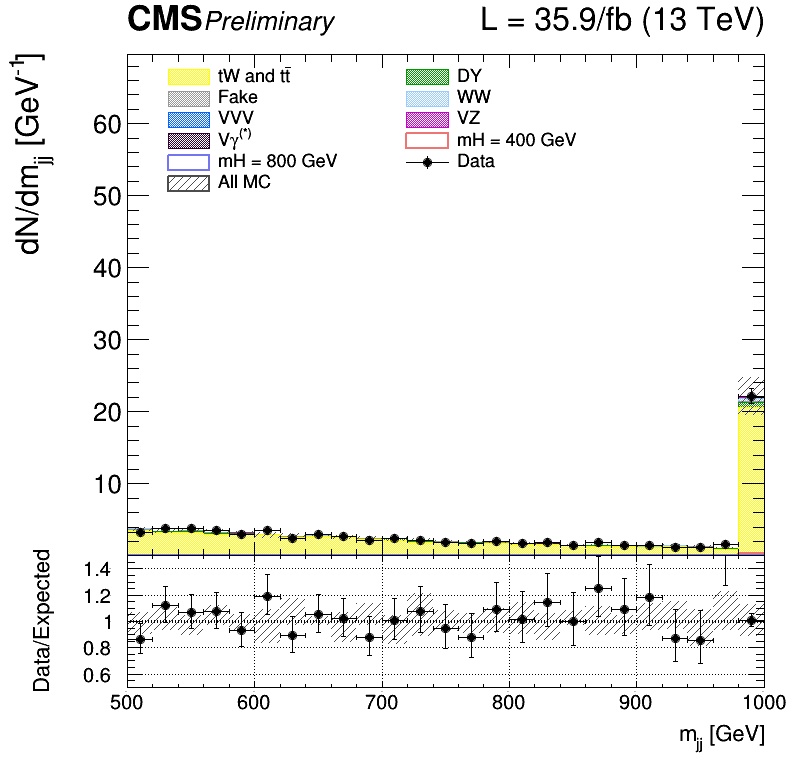
\includegraphics[width=0.45\textwidth]{Figs/SF_CR_Blind/cratio_hww2l2v_13TeV_top_mu_mu_2j_VBF_mjj_DY.png}
}                                              
\subfigure[$m_{\ell \ell}$]{                               
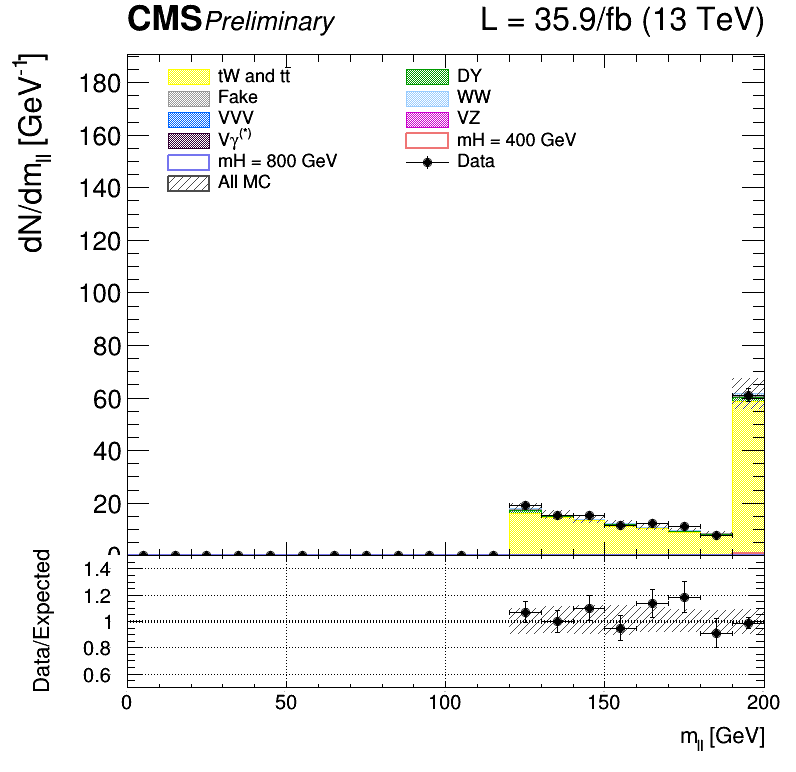
\includegraphics[width=0.45\textwidth]{Figs/SF_CR_Blind/cratio_hww2l2v_13TeV_top_mu_mu_2j_VBF_mll_DY.png}
}\\

\subfigure[$p_T$ leading lepton]{                             
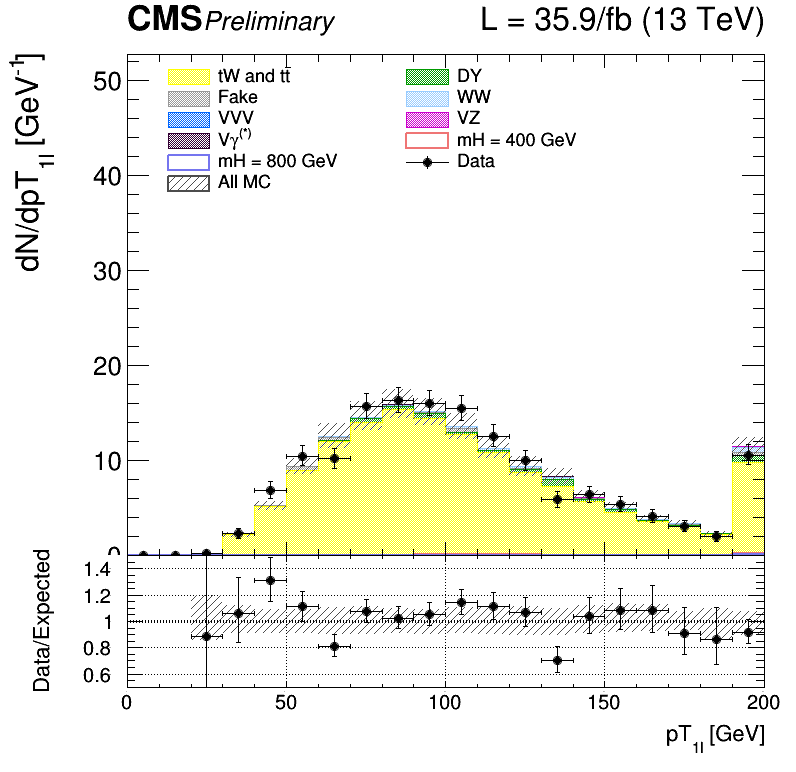
\includegraphics[width=0.45\textwidth]{Figs/SF_CR_Blind/cratio_hww2l2v_13TeV_top_mu_mu_2j_VBF_std_vector_lepton_pt[0].png}
}                                              
\subfigure[$p_T^{\ell \ell}$]{                               
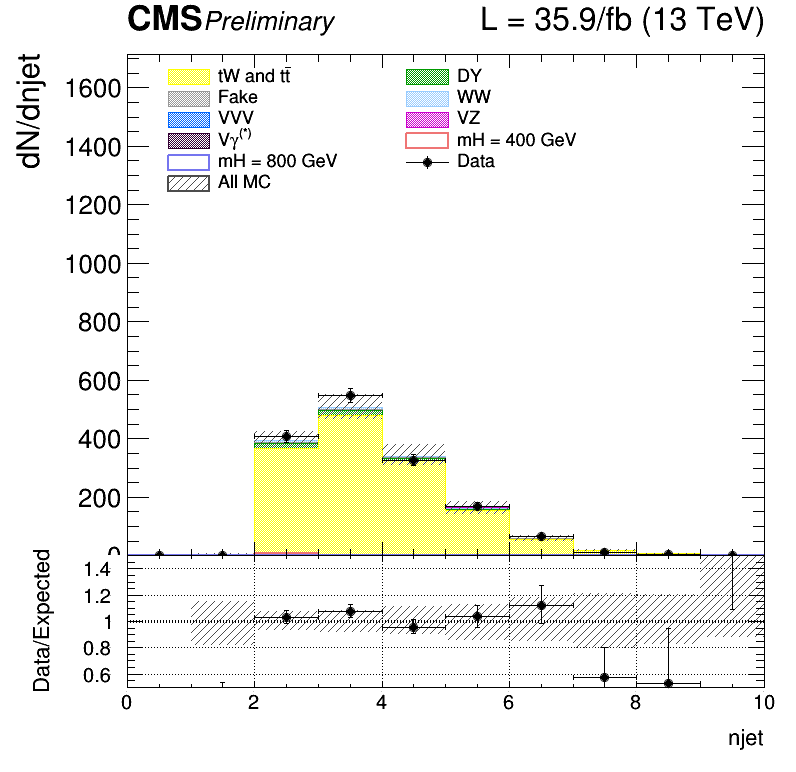
\includegraphics[width=0.45\textwidth]{Figs/SF_CR_Blind/cratio_hww2l2v_13TeV_top_mu_mu_2j_VBF_njet.png}
}\\

\caption{Control plots for several variables in a Top enriched phase space for $\mu \mu$.}
    \label{fig:mll_sigSF_CR_top_mm}
\end{figure}



